\documentclass[nojss]{jss}\usepackage[]{graphicx}\usepackage[]{color}
%% maxwidth is the original width if it is less than linewidth
%% otherwise use linewidth (to make sure the graphics do not exceed the margin)
\makeatletter
\def\maxwidth{ %
  \ifdim\Gin@nat@width>\linewidth
    \linewidth
  \else
    \Gin@nat@width
  \fi
}
\makeatother

\definecolor{fgcolor}{rgb}{0.345, 0.345, 0.345}
\newcommand{\hlnum}[1]{\textcolor[rgb]{0.686,0.059,0.569}{#1}}%
\newcommand{\hlstr}[1]{\textcolor[rgb]{0.192,0.494,0.8}{#1}}%
\newcommand{\hlcom}[1]{\textcolor[rgb]{0.678,0.584,0.686}{\textit{#1}}}%
\newcommand{\hlopt}[1]{\textcolor[rgb]{0,0,0}{#1}}%
\newcommand{\hlstd}[1]{\textcolor[rgb]{0.345,0.345,0.345}{#1}}%
\newcommand{\hlkwa}[1]{\textcolor[rgb]{0.161,0.373,0.58}{\textbf{#1}}}%
\newcommand{\hlkwb}[1]{\textcolor[rgb]{0.69,0.353,0.396}{#1}}%
\newcommand{\hlkwc}[1]{\textcolor[rgb]{0.333,0.667,0.333}{#1}}%
\newcommand{\hlkwd}[1]{\textcolor[rgb]{0.737,0.353,0.396}{\textbf{#1}}}%

\usepackage{framed}
\makeatletter
\newenvironment{kframe}{%
 \def\at@end@of@kframe{}%
 \ifinner\ifhmode%
  \def\at@end@of@kframe{\end{minipage}}%
  \begin{minipage}{\columnwidth}%
 \fi\fi%
 \def\FrameCommand##1{\hskip\@totalleftmargin \hskip-\fboxsep
 \colorbox{shadecolor}{##1}\hskip-\fboxsep
     % There is no \\@totalrightmargin, so:
     \hskip-\linewidth \hskip-\@totalleftmargin \hskip\columnwidth}%
 \MakeFramed {\advance\hsize-\width
   \@totalleftmargin\z@ \linewidth\hsize
   \@setminipage}}%
 {\par\unskip\endMakeFramed%
 \at@end@of@kframe}
\makeatother

\definecolor{shadecolor}{rgb}{.97, .97, .97}
\definecolor{messagecolor}{rgb}{0, 0, 0}
\definecolor{warningcolor}{rgb}{1, 0, 1}
\definecolor{errorcolor}{rgb}{1, 0, 0}
\newenvironment{knitrout}{}{} % an empty environment to be redefined in TeX

\usepackage{alltt}
%\VignetteEngine{knitr::knitr}
%\VignetteIndexEntry{PowerPerformance}

% use examples at http://onepager.togaware.com/KnitRO.pdf
\usepackage{amsmath}

\newcommand{\pname}{PowerPerformance}

%% almost as usual
\author{Andrew Clifton\\ National Renewable Energy Laboratory \And 
Second Author\\Plus Affiliation}

%% for pretty printing and a nice hypersummary also set:
\Plainauthor{Andrew Clifton, Second Author} %% comma-separated
\title{Modeling Wind Turbine Performance with \pname} %% without formatting
\Shorttitle{\pkg{\pname}: Power Performance Modeling} %% a short title (if necessary)

%% an abstract and keywords
\Abstract{
The \pkg{\pname} package includes a variety of functions that are designed to analyze and display wind turbine power performance data. The package also includes methods to model the turbine performance as a function of inflow conditions, including industry-standard approaches, proposed new standard methods, and research tools. Utility functions are also included to quantify and thus compare the accuracy of the different methods. This package accompanies results that were previously published in \cite{Clifton_2013_a} and \cite{Clifton_2013_d}.

At the time of writing, \pkg{\pname} is only available upon request to the author and is supplied without warranty.
}
\Keywords{power curves, wind turbine modeling, machine learning, \proglang{R}}
\Plainkeywords{power curves, wind turbine modeling, machine learning, R} %% without formatting
%% at least one keyword must be supplied

%% The address of (at least) one author should be given
%% in the following format:
\Address{
Andrew Clifton\\
Turbine Modeling and Wind Resource Group\\
National Wind Technology Center\\
National Renewable Energy Laboratory\\
Golden, Colorado, United States of America\\
E-mail: \email{andrew.clifton@nrel.gov}\\
URL: \url{http://http://www.nrel.gov/wind/}
}
\IfFileExists{upquote.sty}{\usepackage{upquote}}{}
\begin{document}
\maketitle



\section{Introduction}
This vignette describes how the \pkg{\pname} package can be used to analyze wind turbine performance data and create different turbine performance models.

\section{Obtaining and installing the package}
The \pkg{\pname} package is currently a developer test version. It is not available through the repositories at \href{http://cran.r-project.org}{CRAN}. To request a copy of the code, please contact \href{mailto:andrew.clifton@nrel.gov}{andrew.clifton@nrel.gov}.

Install \pkg{\pname} and load the package like any other package. To do this in an R client, set the working directory, detach any existing copies of the package, and load the new one:
\begin{knitrout}
\definecolor{shadecolor}{rgb}{0.969, 0.969, 0.969}\color{fgcolor}\begin{kframe}
\begin{alltt}
\hlkwd{setwd}\hlstd{(}\hlstr{"."}\hlstd{)}
\hlkwd{library}\hlstd{(}\hlstr{"PowerPerformance"}\hlstd{)}
\end{alltt}


{\ttfamily\noindent\itshape\color{messagecolor}{\#\# Loading required package: ggplot2\\\#\# Loading required package: randomForest\\\#\# randomForest 4.6-10\\\#\# Type rfNews() to see new features/changes/bug fixes.\\\#\# Loading required package: grid}}\end{kframe}
\end{knitrout}

\pkg{\pname} requires the \href{http://cran.r-project.org/web/packages/randomForest/index.html}{\pkg{randomForest}} and \href{http://cran.r-project.org/web/packages/ggplot2/index.html}{\pkg{ggplot2}} packages. 


\section{Turbine performance data set}
This vignette uses the \code{WindPACT1500kW} data set included in the \pkg{\pname} package. The \code{WindPACT1500kW} data set is a combination of inflow wind and turbine power data from simulations of the Wind Partnership for Advanced Component Technologies 1.5 MW wind turbine. The turbine is described in \citet{Poore_2003_a, Malcolm_32495}. The inflow was simulated using the stochastic wind field modeling tool, Turbsim, to create realistic wind fields for a neutral atmosphere that were then used to force a simulated turbine in the aero-elastic simulator FAST. Data from the inflow simulations and the turbine simulations were post processed using MATLAB to extract 1,524 observations of inflow and turbine response. The process is described in more detail in \citet{Clifton_2013_a} and \citet{Clifton_2013_d}. 

The following variables are included in the \code{WindPACT1500kW} data set:
\begin{description}
\item[\code{ws.HH}]{hub-height wind speed (m/s)}
\item[\code{Ti.HH}]{Turbulence intensity at hub height (\%)}
\item[\code{Shear}]{The exponent of the power law fit to the velocity profile}
\item[\code{ws.eq}]{A rotor-equivalent wind speed (m/s)}
\item[\code{RSS}]{A metric describing the difference between the meaasured velocity profile and an ideal power-law profile}
\item[\code{power.mean}]{The mean power under these conditions (kW)}
\item[\code{power.std}]{The standard deviation of power under these conditions (kW)}
\end{description}

\section{Preparing the data}
\subsection{Loading the data}
The \code{WindPACT1500kW} data are loaded using the \code{data()} function:
\begin{knitrout}
\definecolor{shadecolor}{rgb}{0.969, 0.969, 0.969}\color{fgcolor}\begin{kframe}
\begin{alltt}
\hlkwd{data}\hlstd{(WindPACT1500kW)}
\hlstd{data.in} \hlkwb{<-} \hlstd{WindPACT1500kW}
\end{alltt}
\end{kframe}
\end{knitrout}

We now have all of the variables listed above in a data frame, \code{data.in}. To see what's in there, we'll look at the first three rows of the data frame:

\begin{knitrout}
\definecolor{shadecolor}{rgb}{0.969, 0.969, 0.969}\color{fgcolor}\begin{kframe}
\begin{alltt}
\hlstd{data.in[}\hlnum{1}\hlopt{:}\hlnum{3}\hlstd{,]}
\end{alltt}
\begin{verbatim}
##     ws.HH   Ti.HH    Shear   ws.eq        RSS power.mean power.std
## 1 9.40550 26.3144 0.429427 9.38952 0.01453800   869.8550  362.2920
## 2 6.19517 21.7030 0.414201 6.21101 0.01307880   261.2220  108.6460
## 3 4.03322 35.6918 0.392454 4.05340 0.00404732    79.5682   48.9111
\end{verbatim}
\end{kframe}
\end{knitrout}

\subsection{Data filtering and checking}
The \code{WindPACT1500kW} data are derived from simulations, and thus are more-or-less `perfect'. No filtering is required. However, if a real-world observational data set is being used, the user should be careful to filter the data before use. Check for (at least) the following:

\begin{itemize}
\item The wind is from sectors where there is no effect of tower or turbine wakes, and the cups and vanes or remote sensing devices are not shadowed by the turbine.
\item Wind speeds are within sensible ranges
\item Power is greater than 0 kW
\end{itemize}

To follow the rest of this vignette using your own data, the data should be put into a data frame with the same names as the \code{WindPACT1500kW} data set.

\subsection{Density correction}
If the turbine performance data are derived from simulations or observations that include a range of atmospheric pressure and temperature (and thus density $\rho$), a useful first step may be to adjust the wind speed $u$ to a reference density ($\rho_0$) according to the IEC 61400-12-1 standard. For a turbine with `active power control` or pitch control, this is done by scaling the velocity by the cube root of the density ratio:

\begin{equation}
u_{adj} = u\left(\frac{\rho}{\rho_0}\right)^{1/3}
\end{equation}

This is implemented using the function, \code{PCwsAdjDens()}. Inputs include the wind speed, density associated with that wind speed (in this case fixed at 1.225 kg/m$^3$), and the reference density to use:
\begin{knitrout}
\definecolor{shadecolor}{rgb}{0.969, 0.969, 0.969}\color{fgcolor}\begin{kframe}
\begin{alltt}
\hlstd{data.in}\hlopt{$}\hlstd{ws.HH.adj} \hlkwb{<-} \hlkwd{PCwsAdjDens}\hlstd{(}\hlkwc{ws} \hlstd{= data.in}\hlopt{$}\hlstd{ws.HH,}
                                 \hlkwc{rho} \hlstd{=} \hlnum{1.225}\hlstd{,}
                                 \hlkwc{rho.ref} \hlstd{=} \hlnum{1.225}\hlstd{)}
\end{alltt}
\end{kframe}
\end{knitrout}

\subsection{The rotor-equivalent wind speed}
\cite{wagner_2011_a} suggests accounting for the shear in the inflow by calculating a turbine rotor-disk averaged wind speed and using that in place of the hub-height wind speed. The rotor equivalent wind speed (REWS or $u_{eq}$) is defined as

\begin{equation}
u_{eq} = \sum{u_i^3\frac{A_i}{A}}^{1/3}
\end{equation}

\noindent where $u_i$ is the wind speed in slice $i$, which has area $A_i$.

Given an array of wind speeds at different heights, we can use the \code{GetREWS()} function to calculate the REWS. \code{GetREWS()} divides the rotor disk into horizontal slices between heights $(z_{i-i} + z_{i})/2$ and $(z_i + z_{i+1})/2$ and calculates the area of each slice. The edges of the slices are constrained to the outer radius of the turbine rotor.

\subsection{Turbine operating region}
The turbine operating region (TOR) quantifies how the turbine controls its output power.
\begin{itemize}
\item{Between cut-in and rated wind speed, the turbine is operating at maximum power coefficient. This is known as Region II.}
\item{Between rated and cut-out wind speed, the turbine control system pitches the blades towards feathered to keep the power at the generator's rated power. This is known as Region III.}
\end{itemize}

A convenience function, \code{GetTOR()} is used to code this as a factor:

\begin{knitrout}
\definecolor{shadecolor}{rgb}{0.969, 0.969, 0.969}\color{fgcolor}\begin{kframe}
\begin{alltt}
\hlstd{data.in}\hlopt{$}\hlstd{TOR} \hlkwb{<-} \hlkwd{GetTOR}\hlstd{(data.in}\hlopt{$}\hlstd{ws.HH,}
                      \hlkwc{ws.rated} \hlstd{=} \hlnum{11.5}\hlstd{)}
\hlstd{data.in[}\hlnum{1}\hlstd{,]}
\end{alltt}
\begin{verbatim}
##    ws.HH   Ti.HH    Shear   ws.eq      RSS power.mean power.std ws.HH.adj
## 1 9.4055 26.3144 0.429427 9.38952 0.014538    869.855   362.292    9.4055
##   TOR
## 1  II
\end{verbatim}
\end{kframe}
\end{knitrout}

\subsection{Training and testing data sets}
We'll split the \code{WindPACT1500kW} data into two equal-sized datasets. That gives us a data set to `train' the model, and another to `test' the model that we come up with.

\begin{knitrout}
\definecolor{shadecolor}{rgb}{0.969, 0.969, 0.969}\color{fgcolor}\begin{kframe}
\begin{alltt}
\hlstd{ntrain} \hlkwb{=} \hlkwd{floor}\hlstd{(}\hlkwd{NROW}\hlstd{(data.in)}\hlopt{/}\hlnum{2}\hlstd{)}
\hlstd{train} \hlkwb{=} \hlkwd{rep}\hlstd{(}\hlnum{FALSE}\hlstd{,}\hlkwd{NROW}\hlstd{(data.in))}
\hlstd{train[}\hlkwd{sample}\hlstd{(}\hlkwd{nrow}\hlstd{(data.in), ntrain)]} \hlkwb{=} \hlnum{TRUE}
\hlstd{data.train} \hlkwb{=} \hlstd{data.in[train} \hlopt{==} \hlnum{TRUE}\hlstd{,]}
\hlstd{data.test} \hlkwb{=} \hlstd{data.in[train} \hlopt{==} \hlnum{FALSE}\hlstd{,]}
\end{alltt}
\end{kframe}
\end{knitrout}


\section{Hub-height wind speed power curves}
A power curve is often produced using the `method of binning', whereby the mean power is calculated for 0.5 m/s wind-speed bins. The \code{PCTrainTurbineModel()} function uses the methods described in IEC 61400-12-1 \citep{IEC_61400_12_1} to create the power curve:

\begin{knitrout}
\definecolor{shadecolor}{rgb}{0.969, 0.969, 0.969}\color{fgcolor}\begin{kframe}
\begin{alltt}
\hlstd{PCmodel} \hlkwb{<-} \hlkwd{PCTrainTurbineModel}\hlstd{(}\hlkwc{ws} \hlstd{= data.train}\hlopt{$}\hlstd{ws.HH.adj,}
                               \hlkwc{power} \hlstd{= data.train}\hlopt{$}\hlstd{power.mean)}
\end{alltt}
\end{kframe}
\end{knitrout}

Notice that we use the density-adjusted, hub-height wind speed \code{\$ws.HH.adj} to produce this power curve. If we look at the first few rows of the power curve, we can see the information that it contains:
\begin{knitrout}
\definecolor{shadecolor}{rgb}{0.969, 0.969, 0.969}\color{fgcolor}\begin{kframe}
\begin{alltt}
\hlstd{PCmodel[}\hlnum{1}\hlopt{:}\hlnum{3}\hlstd{,]}
\end{alltt}
\begin{verbatim}
##   ws.binmin ws.binmax ws.binnpoints ws.binmean ti.binmean power.binmean
## 1      0.25      0.75             0        0.5         NA            NA
## 2      0.75      1.25             0        1.0         NA            NA
## 3      1.25      1.75             0        1.5         NA            NA
##   power.binsd
## 1          NA
## 2          NA
## 3          NA
\end{verbatim}
\end{kframe}
\end{knitrout}

We can plot the power curve using \code{plotPC()}, which is a wrapper around a series of \pkg{ggplot2} commands. We can use any of \pkg{ggplot2}'s functions to alter the plot. The power curve in Figure \ref{fig:PCdemo} was generated using \code{plotPC(PC.ws.HH.adj) + theme_bw(base_size = 8)}.

\begin{knitrout}
\definecolor{shadecolor}{rgb}{0.969, 0.969, 0.969}\color{fgcolor}\begin{kframe}


{\ttfamily\noindent\color{warningcolor}{\#\# Warning in loop\_apply(n, do.ply): Removed 5 rows containing missing values (geom\_path).}}

{\ttfamily\noindent\color{warningcolor}{\#\# Warning in loop\_apply(n, do.ply): Removed 5 rows containing missing values (geom\_point).}}\end{kframe}\begin{figure}[h]

{\centering 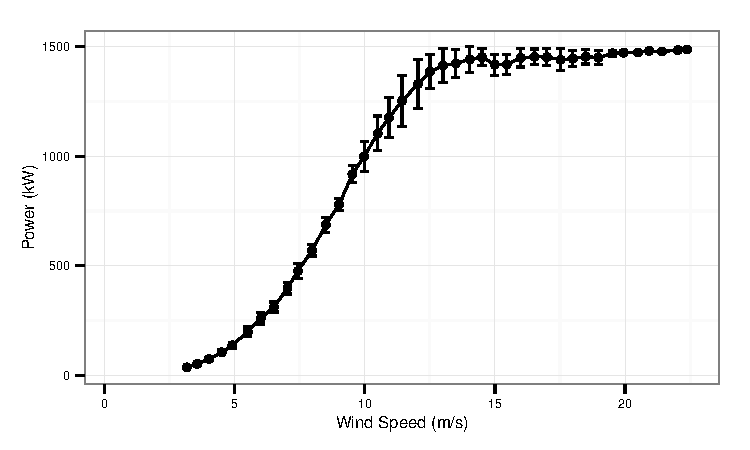
\includegraphics[width=5in,height=3in]{figure/PCdemo-1} 

}

\caption[The power curve derived from the entire WindPACT1500kW data set]{The power curve derived from the entire WindPACT1500kW data set}\label{fig:PCdemo}
\end{figure}


\end{knitrout}

We can query the trained power curve using \code{PCQueryTurbineModel()} to find the power at a given wind speed. In this example we want the power at a wind speed of 10 m/s:
\begin{knitrout}
\definecolor{shadecolor}{rgb}{0.969, 0.969, 0.969}\color{fgcolor}\begin{kframe}
\begin{alltt}
\hlkwd{PCQueryTurbineModel}\hlstd{(}\hlkwc{power.curve} \hlstd{= PCmodel,}
                    \hlkwc{ws} \hlstd{=} \hlnum{10}\hlstd{)}
\end{alltt}
\begin{verbatim}
## [1] 1004.235
\end{verbatim}
\end{kframe}
\end{knitrout}

The problem with the basic power curve is that it doesn't let us account for other effects on power performance than wind speed. the next sections describe some alternative approaches that can add more information in to the power curve.

\section{Zero turbulence power curves}
The zero turbulence power curve has been suggested as a way to quantify the effect of turbulence on the turbine power, and then remove it to find the underlying power curve. The turbulence for a new site can then be added back in to the power curve to give a site-specific power curve. This method is included in the 2014 committee draft of a proposed new IEC 61400-12-1 Power Performance Testing standard.

To start the method, we need a power curve that includes the mean power and the mean turbulence intensity in each of the bins. This can be obtained using \code{PCTrainTurbineModel}:

\begin{knitrout}
\definecolor{shadecolor}{rgb}{0.969, 0.969, 0.969}\color{fgcolor}\begin{kframe}
\begin{alltt}
\hlstd{ZT.init.PC} \hlkwb{<-} \hlkwd{ZTTrainBaselinePCModel}\hlstd{(}\hlkwc{ws} \hlstd{= data.train}\hlopt{$}\hlstd{ws.HH.adj,}
                                     \hlkwc{power} \hlstd{= data.train}\hlopt{$}\hlstd{power.mean,}
                                     \hlkwc{ti} \hlstd{= data.train}\hlopt{$}\hlstd{Ti.HH,}
                                     \hlkwc{ws.cutin} \hlstd{=} \hlnum{2}\hlstd{)}
\end{alltt}
\end{kframe}
\end{knitrout}

Then, we use this power curve to initialize the zero-turbulence power curve. We need to pass in the density at which this power curve was obtained (1.225 kg /m$^3$) and give the turbine diameter, in this case 70 m.

\begin{knitrout}
\definecolor{shadecolor}{rgb}{0.969, 0.969, 0.969}\color{fgcolor}\begin{kframe}
\begin{alltt}
\hlstd{ZT.param} \hlkwb{<-} \hlkwd{ZTTrainInitTurbineModel}\hlstd{(}\hlkwc{PC.values} \hlstd{= ZT.init.PC,}
                                    \hlkwc{rho} \hlstd{=} \hlnum{1.225}\hlstd{,}
                                    \hlkwc{diameter} \hlstd{=} \hlnum{70}\hlstd{)}
\end{alltt}
\end{kframe}
\end{knitrout}

The output from \code{ZTTrainInitTurbineModel()} is used as one of the inputs to \code{ZTTrainTheoTurbineModel()}, along with the bin-mean values of wind speed, turbulence intensity and power from the power curve:

\begin{knitrout}
\definecolor{shadecolor}{rgb}{0.969, 0.969, 0.969}\color{fgcolor}\begin{kframe}
\begin{alltt}
\hlstd{ZT.theo} \hlkwb{<-} \hlkwd{ZTTrainTheoTurbineModel}\hlstd{(}\hlkwc{PC.param} \hlstd{= ZT.param}\hlopt{$}\hlstd{param,}
                                   \hlkwc{ws} \hlstd{= ZT.init.PC}\hlopt{$}\hlstd{ws.binmean,}
                                   \hlkwc{Ti} \hlstd{= ZT.init.PC}\hlopt{$}\hlstd{ti.binmean,}
                                   \hlkwc{power} \hlstd{= ZT.init.PC}\hlopt{$}\hlstd{power.binmean,}
                                   \hlkwc{rho} \hlstd{=} \hlnum{1.225}\hlstd{)}
\end{alltt}
\end{kframe}
\end{knitrout}

Finally, those data are used to calculate the zero-turbulence power curve:

\begin{knitrout}
\definecolor{shadecolor}{rgb}{0.969, 0.969, 0.969}\color{fgcolor}\begin{kframe}
\begin{alltt}
\hlstd{df.PC.zt} \hlkwb{<-} \hlkwd{ZTTrainFinalTurbineModel}\hlstd{(}\hlkwc{PC.param} \hlstd{= ZT.theo}\hlopt{$}\hlstd{param,}
                                     \hlkwc{ws} \hlstd{= data.train}\hlopt{$}\hlstd{ws.HH.adj,}
                                     \hlkwc{Ti} \hlstd{= data.train}\hlopt{$}\hlstd{Ti.HH,}
                                     \hlkwc{power} \hlstd{= data.train}\hlopt{$}\hlstd{power.mean,}
                                     \hlkwc{rho} \hlstd{=} \hlnum{1.225}\hlstd{)}
\end{alltt}
\end{kframe}
\end{knitrout}
And we can plot the power curve that we get, using \code{plotPC(df.PC.zt$values)}:

\begin{knitrout}
\definecolor{shadecolor}{rgb}{0.969, 0.969, 0.969}\color{fgcolor}\begin{kframe}


{\ttfamily\noindent\color{warningcolor}{\#\# Warning in loop\_apply(n, do.ply): Removed 5 rows containing missing values (geom\_path).}}

{\ttfamily\noindent\color{warningcolor}{\#\# Warning in loop\_apply(n, do.ply): Removed 5 rows containing missing values (geom\_point).}}\end{kframe}\begin{figure}[h]

{\centering 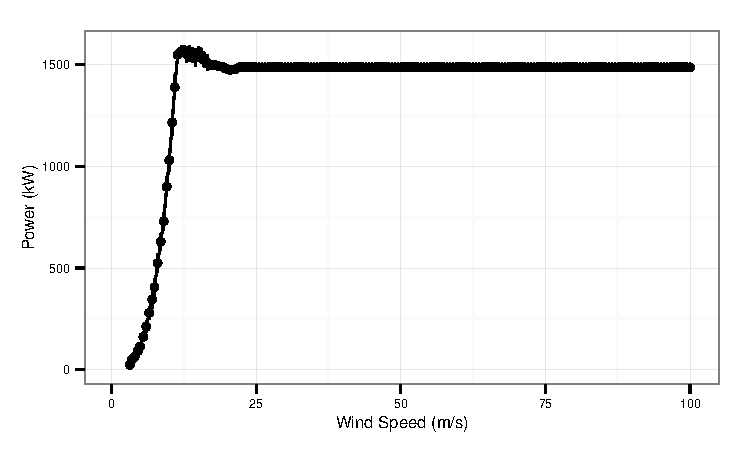
\includegraphics[width=5in,height=3in]{figure/ZTdemo-1} 

}

\caption[The zero-turbulence power curve derived from the WindPACT1500kW data set]{The zero-turbulence power curve derived from the WindPACT1500kW data set}\label{fig:ZTdemo}
\end{figure}


\end{knitrout}

The final step is to add turbulence \emph{back} in, so that we can predict performance for a specific site.

\begin{knitrout}
\definecolor{shadecolor}{rgb}{0.969, 0.969, 0.969}\color{fgcolor}\begin{kframe}
\begin{alltt}
\hlstd{ZTSite} \hlkwb{<-} \hlkwd{data.frame}\hlstd{(}\hlkwc{ws} \hlstd{= data.test}\hlopt{$}\hlstd{ws.HH.adj,}
                     \hlkwc{power} \hlstd{=} \hlkwd{ZTQueryTurbineModel}\hlstd{(}\hlkwc{PC.param} \hlstd{= df.PC.zt}\hlopt{$}\hlstd{param,}
                                                 \hlkwc{ws} \hlstd{= data.train}\hlopt{$}\hlstd{ws.HH.adj,}
                                                 \hlkwc{Ti} \hlstd{= data.train}\hlopt{$}\hlstd{Ti.HH,}
                                                 \hlkwc{power} \hlstd{= data.train}\hlopt{$}\hlstd{power.mean,}
                                                 \hlkwc{rho} \hlstd{=} \hlnum{1.225}\hlstd{,}
                                                 \hlkwc{newTi} \hlstd{= data.test}\hlopt{$}\hlstd{Ti.HH,}
                                                 \hlkwc{newws} \hlstd{= data.test}\hlopt{$}\hlstd{ws.eq))}
\end{alltt}
\begin{verbatim}
## Analyzing point 1 of 762 
## Analyzing point 2 of 762 
## Analyzing point 3 of 762 
## Analyzing point 4 of 762 
## Analyzing point 5 of 762 
## Analyzing point 6 of 762 
## Analyzing point 7 of 762 
## Analyzing point 8 of 762 
## Analyzing point 9 of 762 
## Analyzing point 10 of 762 
## Analyzing point 11 of 762 
## Analyzing point 12 of 762 
## Analyzing point 13 of 762 
## Analyzing point 14 of 762 
## Analyzing point 15 of 762 
## Analyzing point 16 of 762 
## Analyzing point 17 of 762 
## Analyzing point 18 of 762 
## Analyzing point 19 of 762 
## Analyzing point 20 of 762 
## Analyzing point 21 of 762 
## Analyzing point 22 of 762 
## Analyzing point 23 of 762 
## Analyzing point 24 of 762 
## Analyzing point 25 of 762 
## Analyzing point 26 of 762 
## Analyzing point 27 of 762 
## Analyzing point 28 of 762 
## Analyzing point 29 of 762 
## Analyzing point 30 of 762 
## Analyzing point 31 of 762 
## Analyzing point 32 of 762 
## Analyzing point 33 of 762 
## Analyzing point 34 of 762 
## Analyzing point 35 of 762 
## Analyzing point 36 of 762 
## Analyzing point 37 of 762 
## Analyzing point 38 of 762 
## Analyzing point 39 of 762 
## Analyzing point 40 of 762 
## Analyzing point 41 of 762 
## Analyzing point 42 of 762 
## Analyzing point 43 of 762 
## Analyzing point 44 of 762 
## Analyzing point 45 of 762 
## Analyzing point 46 of 762 
## Analyzing point 47 of 762 
## Analyzing point 48 of 762 
## Analyzing point 49 of 762 
## Analyzing point 50 of 762 
## Analyzing point 51 of 762 
## Analyzing point 52 of 762 
## Analyzing point 53 of 762 
## Analyzing point 54 of 762 
## Analyzing point 55 of 762 
## Analyzing point 56 of 762 
## Analyzing point 57 of 762 
## Analyzing point 58 of 762 
## Analyzing point 59 of 762 
## Analyzing point 60 of 762 
## Analyzing point 61 of 762 
## Analyzing point 62 of 762 
## Analyzing point 63 of 762 
## Analyzing point 64 of 762 
## Analyzing point 65 of 762 
## Analyzing point 66 of 762 
## Analyzing point 67 of 762 
## Analyzing point 68 of 762 
## Analyzing point 69 of 762 
## Analyzing point 70 of 762 
## Analyzing point 71 of 762 
## Analyzing point 72 of 762 
## Analyzing point 73 of 762 
## Analyzing point 74 of 762 
## Analyzing point 75 of 762 
## Analyzing point 76 of 762 
## Analyzing point 77 of 762 
## Analyzing point 78 of 762 
## Analyzing point 79 of 762 
## Analyzing point 80 of 762 
## Analyzing point 81 of 762 
## Analyzing point 82 of 762 
## Analyzing point 83 of 762 
## Analyzing point 84 of 762 
## Analyzing point 85 of 762 
## Analyzing point 86 of 762 
## Analyzing point 87 of 762 
## Analyzing point 88 of 762 
## Analyzing point 89 of 762 
## Analyzing point 90 of 762 
## Analyzing point 91 of 762 
## Analyzing point 92 of 762 
## Analyzing point 93 of 762 
## Analyzing point 94 of 762 
## Analyzing point 95 of 762 
## Analyzing point 96 of 762 
## Analyzing point 97 of 762 
## Analyzing point 98 of 762 
## Analyzing point 99 of 762 
## Analyzing point 100 of 762 
## Analyzing point 101 of 762 
## Analyzing point 102 of 762 
## Analyzing point 103 of 762 
## Analyzing point 104 of 762 
## Analyzing point 105 of 762 
## Analyzing point 106 of 762 
## Analyzing point 107 of 762 
## Analyzing point 108 of 762 
## Analyzing point 109 of 762 
## Analyzing point 110 of 762 
## Analyzing point 111 of 762 
## Analyzing point 112 of 762 
## Analyzing point 113 of 762 
## Analyzing point 114 of 762 
## Analyzing point 115 of 762 
## Analyzing point 116 of 762 
## Analyzing point 117 of 762 
## Analyzing point 118 of 762 
## Analyzing point 119 of 762 
## Analyzing point 120 of 762 
## Analyzing point 121 of 762 
## Analyzing point 122 of 762 
## Analyzing point 123 of 762 
## Analyzing point 124 of 762 
## Analyzing point 125 of 762 
## Analyzing point 126 of 762 
## Analyzing point 127 of 762 
## Analyzing point 128 of 762 
## Analyzing point 129 of 762 
## Analyzing point 130 of 762 
## Analyzing point 131 of 762 
## Analyzing point 132 of 762 
## Analyzing point 133 of 762 
## Analyzing point 134 of 762 
## Analyzing point 135 of 762 
## Analyzing point 136 of 762 
## Analyzing point 137 of 762 
## Analyzing point 138 of 762 
## Analyzing point 139 of 762 
## Analyzing point 140 of 762 
## Analyzing point 141 of 762 
## Analyzing point 142 of 762 
## Analyzing point 143 of 762 
## Analyzing point 144 of 762 
## Analyzing point 145 of 762 
## Analyzing point 146 of 762 
## Analyzing point 147 of 762 
## Analyzing point 148 of 762 
## Analyzing point 149 of 762 
## Analyzing point 150 of 762 
## Analyzing point 151 of 762 
## Analyzing point 152 of 762 
## Analyzing point 153 of 762 
## Analyzing point 154 of 762 
## Analyzing point 155 of 762 
## Analyzing point 156 of 762 
## Analyzing point 157 of 762 
## Analyzing point 158 of 762 
## Analyzing point 159 of 762 
## Analyzing point 160 of 762 
## Analyzing point 161 of 762 
## Analyzing point 162 of 762 
## Analyzing point 163 of 762 
## Analyzing point 164 of 762 
## Analyzing point 165 of 762 
## Analyzing point 166 of 762 
## Analyzing point 167 of 762 
## Analyzing point 168 of 762 
## Analyzing point 169 of 762 
## Analyzing point 170 of 762 
## Analyzing point 171 of 762 
## Analyzing point 172 of 762 
## Analyzing point 173 of 762 
## Analyzing point 174 of 762 
## Analyzing point 175 of 762 
## Analyzing point 176 of 762 
## Analyzing point 177 of 762 
## Analyzing point 178 of 762 
## Analyzing point 179 of 762 
## Analyzing point 180 of 762 
## Analyzing point 181 of 762 
## Analyzing point 182 of 762 
## Analyzing point 183 of 762 
## Analyzing point 184 of 762 
## Analyzing point 185 of 762 
## Analyzing point 186 of 762 
## Analyzing point 187 of 762 
## Analyzing point 188 of 762 
## Analyzing point 189 of 762 
## Analyzing point 190 of 762 
## Analyzing point 191 of 762 
## Analyzing point 192 of 762 
## Analyzing point 193 of 762 
## Analyzing point 194 of 762 
## Analyzing point 195 of 762 
## Analyzing point 196 of 762 
## Analyzing point 197 of 762 
## Analyzing point 198 of 762 
## Analyzing point 199 of 762 
## Analyzing point 200 of 762 
## Analyzing point 201 of 762 
## Analyzing point 202 of 762 
## Analyzing point 203 of 762 
## Analyzing point 204 of 762 
## Analyzing point 205 of 762 
## Analyzing point 206 of 762 
## Analyzing point 207 of 762 
## Analyzing point 208 of 762 
## Analyzing point 209 of 762 
## Analyzing point 210 of 762 
## Analyzing point 211 of 762 
## Analyzing point 212 of 762 
## Analyzing point 213 of 762 
## Analyzing point 214 of 762 
## Analyzing point 215 of 762 
## Analyzing point 216 of 762 
## Analyzing point 217 of 762 
## Analyzing point 218 of 762 
## Analyzing point 219 of 762 
## Analyzing point 220 of 762 
## Analyzing point 221 of 762 
## Analyzing point 222 of 762 
## Analyzing point 223 of 762 
## Analyzing point 224 of 762 
## Analyzing point 225 of 762 
## Analyzing point 226 of 762 
## Analyzing point 227 of 762 
## Analyzing point 228 of 762 
## Analyzing point 229 of 762 
## Analyzing point 230 of 762 
## Analyzing point 231 of 762 
## Analyzing point 232 of 762 
## Analyzing point 233 of 762 
## Analyzing point 234 of 762 
## Analyzing point 235 of 762 
## Analyzing point 236 of 762 
## Analyzing point 237 of 762 
## Analyzing point 238 of 762 
## Analyzing point 239 of 762 
## Analyzing point 240 of 762 
## Analyzing point 241 of 762 
## Analyzing point 242 of 762 
## Analyzing point 243 of 762 
## Analyzing point 244 of 762 
## Analyzing point 245 of 762 
## Analyzing point 246 of 762 
## Analyzing point 247 of 762 
## Analyzing point 248 of 762 
## Analyzing point 249 of 762 
## Analyzing point 250 of 762 
## Analyzing point 251 of 762 
## Analyzing point 252 of 762 
## Analyzing point 253 of 762 
## Analyzing point 254 of 762 
## Analyzing point 255 of 762 
## Analyzing point 256 of 762 
## Analyzing point 257 of 762 
## Analyzing point 258 of 762 
## Analyzing point 259 of 762 
## Analyzing point 260 of 762 
## Analyzing point 261 of 762 
## Analyzing point 262 of 762 
## Analyzing point 263 of 762 
## Analyzing point 264 of 762 
## Analyzing point 265 of 762 
## Analyzing point 266 of 762 
## Analyzing point 267 of 762 
## Analyzing point 268 of 762 
## Analyzing point 269 of 762 
## Analyzing point 270 of 762 
## Analyzing point 271 of 762 
## Analyzing point 272 of 762 
## Analyzing point 273 of 762 
## Analyzing point 274 of 762 
## Analyzing point 275 of 762 
## Analyzing point 276 of 762 
## Analyzing point 277 of 762 
## Analyzing point 278 of 762 
## Analyzing point 279 of 762 
## Analyzing point 280 of 762 
## Analyzing point 281 of 762 
## Analyzing point 282 of 762 
## Analyzing point 283 of 762 
## Analyzing point 284 of 762 
## Analyzing point 285 of 762 
## Analyzing point 286 of 762 
## Analyzing point 287 of 762 
## Analyzing point 288 of 762 
## Analyzing point 289 of 762 
## Analyzing point 290 of 762 
## Analyzing point 291 of 762 
## Analyzing point 292 of 762 
## Analyzing point 293 of 762 
## Analyzing point 294 of 762 
## Analyzing point 295 of 762 
## Analyzing point 296 of 762 
## Analyzing point 297 of 762 
## Analyzing point 298 of 762 
## Analyzing point 299 of 762 
## Analyzing point 300 of 762 
## Analyzing point 301 of 762 
## Analyzing point 302 of 762 
## Analyzing point 303 of 762 
## Analyzing point 304 of 762 
## Analyzing point 305 of 762 
## Analyzing point 306 of 762 
## Analyzing point 307 of 762 
## Analyzing point 308 of 762 
## Analyzing point 309 of 762 
## Analyzing point 310 of 762 
## Analyzing point 311 of 762 
## Analyzing point 312 of 762 
## Analyzing point 313 of 762 
## Analyzing point 314 of 762 
## Analyzing point 315 of 762 
## Analyzing point 316 of 762 
## Analyzing point 317 of 762 
## Analyzing point 318 of 762 
## Analyzing point 319 of 762 
## Analyzing point 320 of 762 
## Analyzing point 321 of 762 
## Analyzing point 322 of 762 
## Analyzing point 323 of 762 
## Analyzing point 324 of 762 
## Analyzing point 325 of 762 
## Analyzing point 326 of 762 
## Analyzing point 327 of 762 
## Analyzing point 328 of 762 
## Analyzing point 329 of 762 
## Analyzing point 330 of 762 
## Analyzing point 331 of 762 
## Analyzing point 332 of 762 
## Analyzing point 333 of 762 
## Analyzing point 334 of 762 
## Analyzing point 335 of 762 
## Analyzing point 336 of 762 
## Analyzing point 337 of 762 
## Analyzing point 338 of 762 
## Analyzing point 339 of 762 
## Analyzing point 340 of 762 
## Analyzing point 341 of 762 
## Analyzing point 342 of 762 
## Analyzing point 343 of 762 
## Analyzing point 344 of 762 
## Analyzing point 345 of 762 
## Analyzing point 346 of 762 
## Analyzing point 347 of 762 
## Analyzing point 348 of 762 
## Analyzing point 349 of 762 
## Analyzing point 350 of 762 
## Analyzing point 351 of 762 
## Analyzing point 352 of 762 
## Analyzing point 353 of 762 
## Analyzing point 354 of 762 
## Analyzing point 355 of 762 
## Analyzing point 356 of 762 
## Analyzing point 357 of 762 
## Analyzing point 358 of 762 
## Analyzing point 359 of 762 
## Analyzing point 360 of 762 
## Analyzing point 361 of 762 
## Analyzing point 362 of 762 
## Analyzing point 363 of 762 
## Analyzing point 364 of 762 
## Analyzing point 365 of 762 
## Analyzing point 366 of 762 
## Analyzing point 367 of 762 
## Analyzing point 368 of 762 
## Analyzing point 369 of 762 
## Analyzing point 370 of 762 
## Analyzing point 371 of 762 
## Analyzing point 372 of 762 
## Analyzing point 373 of 762 
## Analyzing point 374 of 762 
## Analyzing point 375 of 762 
## Analyzing point 376 of 762 
## Analyzing point 377 of 762 
## Analyzing point 378 of 762 
## Analyzing point 379 of 762 
## Analyzing point 380 of 762 
## Analyzing point 381 of 762 
## Analyzing point 382 of 762 
## Analyzing point 383 of 762 
## Analyzing point 384 of 762 
## Analyzing point 385 of 762 
## Analyzing point 386 of 762 
## Analyzing point 387 of 762 
## Analyzing point 388 of 762 
## Analyzing point 389 of 762 
## Analyzing point 390 of 762 
## Analyzing point 391 of 762 
## Analyzing point 392 of 762 
## Analyzing point 393 of 762 
## Analyzing point 394 of 762 
## Analyzing point 395 of 762 
## Analyzing point 396 of 762 
## Analyzing point 397 of 762 
## Analyzing point 398 of 762 
## Analyzing point 399 of 762 
## Analyzing point 400 of 762 
## Analyzing point 401 of 762 
## Analyzing point 402 of 762 
## Analyzing point 403 of 762 
## Analyzing point 404 of 762 
## Analyzing point 405 of 762 
## Analyzing point 406 of 762 
## Analyzing point 407 of 762 
## Analyzing point 408 of 762 
## Analyzing point 409 of 762 
## Analyzing point 410 of 762 
## Analyzing point 411 of 762 
## Analyzing point 412 of 762 
## Analyzing point 413 of 762 
## Analyzing point 414 of 762 
## Analyzing point 415 of 762 
## Analyzing point 416 of 762 
## Analyzing point 417 of 762 
## Analyzing point 418 of 762 
## Analyzing point 419 of 762 
## Analyzing point 420 of 762 
## Analyzing point 421 of 762 
## Analyzing point 422 of 762 
## Analyzing point 423 of 762 
## Analyzing point 424 of 762 
## Analyzing point 425 of 762 
## Analyzing point 426 of 762 
## Analyzing point 427 of 762 
## Analyzing point 428 of 762 
## Analyzing point 429 of 762 
## Analyzing point 430 of 762 
## Analyzing point 431 of 762 
## Analyzing point 432 of 762 
## Analyzing point 433 of 762 
## Analyzing point 434 of 762 
## Analyzing point 435 of 762 
## Analyzing point 436 of 762 
## Analyzing point 437 of 762 
## Analyzing point 438 of 762 
## Analyzing point 439 of 762 
## Analyzing point 440 of 762 
## Analyzing point 441 of 762 
## Analyzing point 442 of 762 
## Analyzing point 443 of 762 
## Analyzing point 444 of 762 
## Analyzing point 445 of 762 
## Analyzing point 446 of 762 
## Analyzing point 447 of 762 
## Analyzing point 448 of 762 
## Analyzing point 449 of 762 
## Analyzing point 450 of 762 
## Analyzing point 451 of 762 
## Analyzing point 452 of 762 
## Analyzing point 453 of 762 
## Analyzing point 454 of 762 
## Analyzing point 455 of 762 
## Analyzing point 456 of 762 
## Analyzing point 457 of 762 
## Analyzing point 458 of 762 
## Analyzing point 459 of 762 
## Analyzing point 460 of 762 
## Analyzing point 461 of 762 
## Analyzing point 462 of 762 
## Analyzing point 463 of 762 
## Analyzing point 464 of 762 
## Analyzing point 465 of 762 
## Analyzing point 466 of 762 
## Analyzing point 467 of 762 
## Analyzing point 468 of 762 
## Analyzing point 469 of 762 
## Analyzing point 470 of 762 
## Analyzing point 471 of 762 
## Analyzing point 472 of 762 
## Analyzing point 473 of 762 
## Analyzing point 474 of 762 
## Analyzing point 475 of 762 
## Analyzing point 476 of 762 
## Analyzing point 477 of 762 
## Analyzing point 478 of 762 
## Analyzing point 479 of 762 
## Analyzing point 480 of 762 
## Analyzing point 481 of 762 
## Analyzing point 482 of 762 
## Analyzing point 483 of 762 
## Analyzing point 484 of 762 
## Analyzing point 485 of 762 
## Analyzing point 486 of 762 
## Analyzing point 487 of 762 
## Analyzing point 488 of 762 
## Analyzing point 489 of 762 
## Analyzing point 490 of 762 
## Analyzing point 491 of 762 
## Analyzing point 492 of 762 
## Analyzing point 493 of 762 
## Analyzing point 494 of 762 
## Analyzing point 495 of 762 
## Analyzing point 496 of 762 
## Analyzing point 497 of 762 
## Analyzing point 498 of 762 
## Analyzing point 499 of 762 
## Analyzing point 500 of 762 
## Analyzing point 501 of 762 
## Analyzing point 502 of 762 
## Analyzing point 503 of 762 
## Analyzing point 504 of 762 
## Analyzing point 505 of 762 
## Analyzing point 506 of 762 
## Analyzing point 507 of 762 
## Analyzing point 508 of 762 
## Analyzing point 509 of 762 
## Analyzing point 510 of 762 
## Analyzing point 511 of 762 
## Analyzing point 512 of 762 
## Analyzing point 513 of 762 
## Analyzing point 514 of 762 
## Analyzing point 515 of 762 
## Analyzing point 516 of 762 
## Analyzing point 517 of 762 
## Analyzing point 518 of 762 
## Analyzing point 519 of 762 
## Analyzing point 520 of 762 
## Analyzing point 521 of 762 
## Analyzing point 522 of 762 
## Analyzing point 523 of 762 
## Analyzing point 524 of 762 
## Analyzing point 525 of 762 
## Analyzing point 526 of 762 
## Analyzing point 527 of 762 
## Analyzing point 528 of 762 
## Analyzing point 529 of 762 
## Analyzing point 530 of 762 
## Analyzing point 531 of 762 
## Analyzing point 532 of 762 
## Analyzing point 533 of 762 
## Analyzing point 534 of 762 
## Analyzing point 535 of 762 
## Analyzing point 536 of 762 
## Analyzing point 537 of 762 
## Analyzing point 538 of 762 
## Analyzing point 539 of 762 
## Analyzing point 540 of 762 
## Analyzing point 541 of 762 
## Analyzing point 542 of 762 
## Analyzing point 543 of 762 
## Analyzing point 544 of 762 
## Analyzing point 545 of 762 
## Analyzing point 546 of 762 
## Analyzing point 547 of 762 
## Analyzing point 548 of 762 
## Analyzing point 549 of 762 
## Analyzing point 550 of 762 
## Analyzing point 551 of 762 
## Analyzing point 552 of 762 
## Analyzing point 553 of 762 
## Analyzing point 554 of 762 
## Analyzing point 555 of 762 
## Analyzing point 556 of 762 
## Analyzing point 557 of 762 
## Analyzing point 558 of 762 
## Analyzing point 559 of 762 
## Analyzing point 560 of 762 
## Analyzing point 561 of 762 
## Analyzing point 562 of 762 
## Analyzing point 563 of 762 
## Analyzing point 564 of 762 
## Analyzing point 565 of 762 
## Analyzing point 566 of 762 
## Analyzing point 567 of 762 
## Analyzing point 568 of 762 
## Analyzing point 569 of 762 
## Analyzing point 570 of 762 
## Analyzing point 571 of 762 
## Analyzing point 572 of 762 
## Analyzing point 573 of 762 
## Analyzing point 574 of 762 
## Analyzing point 575 of 762 
## Analyzing point 576 of 762 
## Analyzing point 577 of 762 
## Analyzing point 578 of 762 
## Analyzing point 579 of 762 
## Analyzing point 580 of 762 
## Analyzing point 581 of 762 
## Analyzing point 582 of 762 
## Analyzing point 583 of 762 
## Analyzing point 584 of 762 
## Analyzing point 585 of 762 
## Analyzing point 586 of 762 
## Analyzing point 587 of 762 
## Analyzing point 588 of 762 
## Analyzing point 589 of 762 
## Analyzing point 590 of 762 
## Analyzing point 591 of 762 
## Analyzing point 592 of 762 
## Analyzing point 593 of 762 
## Analyzing point 594 of 762 
## Analyzing point 595 of 762 
## Analyzing point 596 of 762 
## Analyzing point 597 of 762 
## Analyzing point 598 of 762 
## Analyzing point 599 of 762 
## Analyzing point 600 of 762 
## Analyzing point 601 of 762 
## Analyzing point 602 of 762 
## Analyzing point 603 of 762 
## Analyzing point 604 of 762 
## Analyzing point 605 of 762 
## Analyzing point 606 of 762 
## Analyzing point 607 of 762 
## Analyzing point 608 of 762 
## Analyzing point 609 of 762 
## Analyzing point 610 of 762 
## Analyzing point 611 of 762 
## Analyzing point 612 of 762 
## Analyzing point 613 of 762 
## Analyzing point 614 of 762 
## Analyzing point 615 of 762 
## Analyzing point 616 of 762 
## Analyzing point 617 of 762 
## Analyzing point 618 of 762 
## Analyzing point 619 of 762 
## Analyzing point 620 of 762 
## Analyzing point 621 of 762 
## Analyzing point 622 of 762 
## Analyzing point 623 of 762 
## Analyzing point 624 of 762 
## Analyzing point 625 of 762 
## Analyzing point 626 of 762 
## Analyzing point 627 of 762 
## Analyzing point 628 of 762 
## Analyzing point 629 of 762 
## Analyzing point 630 of 762 
## Analyzing point 631 of 762 
## Analyzing point 632 of 762 
## Analyzing point 633 of 762 
## Analyzing point 634 of 762 
## Analyzing point 635 of 762 
## Analyzing point 636 of 762 
## Analyzing point 637 of 762 
## Analyzing point 638 of 762 
## Analyzing point 639 of 762 
## Analyzing point 640 of 762 
## Analyzing point 641 of 762 
## Analyzing point 642 of 762 
## Analyzing point 643 of 762 
## Analyzing point 644 of 762 
## Analyzing point 645 of 762 
## Analyzing point 646 of 762 
## Analyzing point 647 of 762 
## Analyzing point 648 of 762 
## Analyzing point 649 of 762 
## Analyzing point 650 of 762 
## Analyzing point 651 of 762 
## Analyzing point 652 of 762 
## Analyzing point 653 of 762 
## Analyzing point 654 of 762 
## Analyzing point 655 of 762 
## Analyzing point 656 of 762 
## Analyzing point 657 of 762 
## Analyzing point 658 of 762 
## Analyzing point 659 of 762 
## Analyzing point 660 of 762 
## Analyzing point 661 of 762 
## Analyzing point 662 of 762 
## Analyzing point 663 of 762 
## Analyzing point 664 of 762 
## Analyzing point 665 of 762 
## Analyzing point 666 of 762 
## Analyzing point 667 of 762 
## Analyzing point 668 of 762 
## Analyzing point 669 of 762 
## Analyzing point 670 of 762 
## Analyzing point 671 of 762 
## Analyzing point 672 of 762 
## Analyzing point 673 of 762 
## Analyzing point 674 of 762 
## Analyzing point 675 of 762 
## Analyzing point 676 of 762 
## Analyzing point 677 of 762 
## Analyzing point 678 of 762 
## Analyzing point 679 of 762 
## Analyzing point 680 of 762 
## Analyzing point 681 of 762 
## Analyzing point 682 of 762 
## Analyzing point 683 of 762 
## Analyzing point 684 of 762 
## Analyzing point 685 of 762 
## Analyzing point 686 of 762 
## Analyzing point 687 of 762 
## Analyzing point 688 of 762 
## Analyzing point 689 of 762 
## Analyzing point 690 of 762 
## Analyzing point 691 of 762 
## Analyzing point 692 of 762 
## Analyzing point 693 of 762 
## Analyzing point 694 of 762 
## Analyzing point 695 of 762 
## Analyzing point 696 of 762 
## Analyzing point 697 of 762 
## Analyzing point 698 of 762 
## Analyzing point 699 of 762 
## Analyzing point 700 of 762 
## Analyzing point 701 of 762 
## Analyzing point 702 of 762 
## Analyzing point 703 of 762 
## Analyzing point 704 of 762 
## Analyzing point 705 of 762 
## Analyzing point 706 of 762 
## Analyzing point 707 of 762 
## Analyzing point 708 of 762 
## Analyzing point 709 of 762 
## Analyzing point 710 of 762 
## Analyzing point 711 of 762 
## Analyzing point 712 of 762 
## Analyzing point 713 of 762 
## Analyzing point 714 of 762 
## Analyzing point 715 of 762 
## Analyzing point 716 of 762 
## Analyzing point 717 of 762 
## Analyzing point 718 of 762 
## Analyzing point 719 of 762 
## Analyzing point 720 of 762 
## Analyzing point 721 of 762 
## Analyzing point 722 of 762 
## Analyzing point 723 of 762 
## Analyzing point 724 of 762 
## Analyzing point 725 of 762 
## Analyzing point 726 of 762 
## Analyzing point 727 of 762 
## Analyzing point 728 of 762 
## Analyzing point 729 of 762 
## Analyzing point 730 of 762 
## Analyzing point 731 of 762 
## Analyzing point 732 of 762 
## Analyzing point 733 of 762 
## Analyzing point 734 of 762 
## Analyzing point 735 of 762 
## Analyzing point 736 of 762 
## Analyzing point 737 of 762 
## Analyzing point 738 of 762 
## Analyzing point 739 of 762 
## Analyzing point 740 of 762 
## Analyzing point 741 of 762 
## Analyzing point 742 of 762 
## Analyzing point 743 of 762 
## Analyzing point 744 of 762 
## Analyzing point 745 of 762 
## Analyzing point 746 of 762 
## Analyzing point 747 of 762 
## Analyzing point 748 of 762 
## Analyzing point 749 of 762 
## Analyzing point 750 of 762 
## Analyzing point 751 of 762 
## Analyzing point 752 of 762 
## Analyzing point 753 of 762 
## Analyzing point 754 of 762 
## Analyzing point 755 of 762 
## Analyzing point 756 of 762 
## Analyzing point 757 of 762 
## Analyzing point 758 of 762 
## Analyzing point 759 of 762 
## Analyzing point 760 of 762 
## Analyzing point 761 of 762 
## Analyzing point 762 of 762
\end{verbatim}
\end{kframe}
\end{knitrout}

\section{Multivariate power curves using random forests}
\pkg{\pname} also includes interfaces to a multivariate modeling method called `random forests`, which are coded in the package \pkg{randomForest} \citep{Liaw_2002_a}. Random forests allow many different inputs (continuous or categorical) to be used to estimate a single output. Random forests have been used to predict turbine power output by \cite{Clifton_2013_a, Clifton_2013_d}.

\subsection{Creating a random forest model}
Our first random forest model will include variables from the \code{WindPACT1500kW} data set that describe the kinetic energy through the rotor disk (\code{\$ws.HH.adj}), the variability of that energy (\code{\$Ti.HH}), the shear exponent (\code{\$Shear}), and the turbine operating region \code{\$TOR}. The variable we want to predict is the mean power in a 10-minute interval, \code{\$power.mean}.

We can now make data frames for the training and testing data sets. Both the training and testing data set will contain predictors and a response, and need to contain exactly the same variables.
\begin{knitrout}
\definecolor{shadecolor}{rgb}{0.969, 0.969, 0.969}\color{fgcolor}\begin{kframe}
\begin{alltt}
\hlstd{train.predictors} \hlkwb{=} \hlkwd{data.frame}\hlstd{(}\hlstr{"ws.HH"} \hlstd{= data.train}\hlopt{$}\hlstd{ws.HH.adj,}
                              \hlstr{"ti"} \hlstd{= data.train}\hlopt{$}\hlstd{Ti.HH,}
                              \hlstr{"shear"} \hlstd{= data.train}\hlopt{$}\hlstd{Shear,}
                              \hlstr{"TOR"} \hlstd{= data.train}\hlopt{$}\hlstd{TOR)}
\hlstd{train.response} \hlkwb{=} \hlstd{data.train}\hlopt{$}\hlstd{power.mean}
\hlstd{test.predictors} \hlkwb{=} \hlkwd{data.frame}\hlstd{(}\hlstr{"ws.HH"} \hlstd{= data.test}\hlopt{$}\hlstd{ws.HH.adj,}
                             \hlstr{"ti"} \hlstd{= data.test}\hlopt{$}\hlstd{Ti.HH,}
                             \hlstr{"shear"} \hlstd{= data.test}\hlopt{$}\hlstd{Shear,}
                             \hlstr{"TOR"} \hlstd{= data.test}\hlopt{$}\hlstd{TOR)}
\hlstd{test.response} \hlkwb{=} \hlstd{data.test}\hlopt{$}\hlstd{power.mean}
\end{alltt}
\end{kframe}
\end{knitrout}

We can confirm that both data frame contain the same variable names with the \code{names()} function:
\begin{knitrout}
\definecolor{shadecolor}{rgb}{0.969, 0.969, 0.969}\color{fgcolor}\begin{kframe}
\begin{alltt}
\hlkwd{names}\hlstd{(train.predictors)}
\end{alltt}
\begin{verbatim}
## [1] "ws.HH" "ti"    "shear" "TOR"
\end{verbatim}
\begin{alltt}
\hlkwd{names}\hlstd{(test.predictors)}
\end{alltt}
\begin{verbatim}
## [1] "ws.HH" "ti"    "shear" "TOR"
\end{verbatim}
\end{kframe}
\end{knitrout}

Now, working with the training data, we'll train our random forest-based model. We need to pass in the data frames of training data for the predictive variables, and the response.

\begin{knitrout}
\definecolor{shadecolor}{rgb}{0.969, 0.969, 0.969}\color{fgcolor}\begin{kframe}
\begin{alltt}
\hlstd{RFmodel} \hlkwb{<-} \hlkwd{RFTrainTurbineModel}\hlstd{(}\hlkwc{predictors} \hlstd{= train.predictors,}
                               \hlkwc{response} \hlstd{= train.response)}
\end{alltt}
\end{kframe}
\end{knitrout}

Our random forest model is now ready for use.

\subsection{Querying the random forest model}
Now that we have a model of the turbine, we can query it to find the predicted response to a new set of conditions using \code{RFQueryTurbineModel()}. We can use the first row of the test data set to illustrate this.

\begin{knitrout}
\definecolor{shadecolor}{rgb}{0.969, 0.969, 0.969}\color{fgcolor}\begin{kframe}
\begin{alltt}
\hlkwd{RFQueryTurbineModel}\hlstd{(}\hlkwc{predictors} \hlstd{= test.predictors[}\hlnum{1}\hlstd{,],}
                    \hlkwc{model} \hlstd{= RFmodel)}
\end{alltt}
\begin{verbatim}
##       mean     sdev
## 1 899.0942 74.93374
\end{verbatim}
\end{kframe}
\end{knitrout}

It is very important that the data frame we use to query the model (the \code{predictors = ...} argument) has exactly the same names as the training data set.

We can limit our query to the mean power, too:
\begin{knitrout}
\definecolor{shadecolor}{rgb}{0.969, 0.969, 0.969}\color{fgcolor}\begin{kframe}
\begin{alltt}
\hlkwd{RFQueryTurbineModel}\hlstd{(}\hlkwc{predictors} \hlstd{= test.predictors[}\hlnum{1}\hlstd{,],}
                    \hlkwc{model} \hlstd{= RFmodel)}\hlopt{$}\hlstd{mean}
\end{alltt}
\begin{verbatim}
## [1] 899.0942
\end{verbatim}
\end{kframe}
\end{knitrout}

A convenience function \code{RFTrainTestTurbineModel} combines the training and testing of the RF model, and outputs the results.

\begin{knitrout}
\definecolor{shadecolor}{rgb}{0.969, 0.969, 0.969}\color{fgcolor}\begin{kframe}
\begin{alltt}
\hlkwd{RFTrainTestTurbineModel}\hlstd{(train.predictors,}
                        \hlstd{train.response,}
                        \hlstd{test.predictors,}
                        \hlstd{test.response)}
\end{alltt}
\begin{verbatim}
## $model
## 
## Call:
##  randomForest(x = predictors, y = response, ntree = ntree, mtry = 2,      replace = TRUE, na.action = na.omit) 
##                Type of random forest: regression
##                      Number of trees: 1001
## No. of variables tried at each split: 2
## 
##           Mean of squared residuals: 527.8949
##                     % Var explained: 99.82
## 
## $metrics
##                 metric               type        value
## 1  Pearson Correlation       Error metric 9.989240e-01
## 2                 RMSE       Error metric 2.481356e+01
## 3              Max(AE)       Error metric 1.810967e+02
## 4                  MAE       Error metric 1.421059e+01
## 5                  SAE       Error metric 1.082847e+04
## 6                  SPE       Error metric 6.043756e+03
## 7        Training time Performance metric 1.422000e+00
## 8         Testing time Performance metric 1.990000e-01
## 9                ws.HH  Importance metric 1.528191e+08
## 10                  ti  Importance metric 2.905333e+06
## 11               shear  Importance metric 2.589167e+06
## 12                 TOR  Importance metric 6.503670e+07
\end{verbatim}
\end{kframe}
\end{knitrout}

\subsection{Creating custom random forest models}
There are some important things to remember when putting the random forest model together:
\begin{enumerate}
\item The model can be used to predict any single variable as a function of any input. For example, \cite{Clifton_2013_d} shows that it may be possible to predict loads at a turbine deployment site as a function of wind speed, turbulence, and shear using a random forest model trained by high-fidelity simulations.
\item The same variable names need to be present in the training data frame and the testing data frame.
\item Models should be realistic. Use variables that are important for the turbine response. For the power, that would suggest data that describe the kinetic energy through the rotor disk, the variability of that inflow, and the ability of the turbine to harvest that energy. Also, a variable that describes the turbine controller may help - this could be as simple as the operating region, or possibly some constants within the controller. 
\end{enumerate}

\subsection{Limitations of the random forest method}
The chief limitation of the random forest method is that it requires the model to be trained with data that encompass the likely range of new cases. This is because the model is a statistically-based approach, rather than physics-based. For example, if the model is only trained with data where wind speeds are less than 10 m/s, a prediction at 12 m/s would be unwise. However, given knowledge of a turbine's rotor size, rated speed, and rated power, an engineer would be able to estimate the likely power at this new wind speed (albeit roughly).

\section{Comparing models}
We can test how accurate the different models are, compared to each other. First, we create a new data frame and add a column for the observed power in the testing data frame:

\begin{knitrout}
\definecolor{shadecolor}{rgb}{0.969, 0.969, 0.969}\color{fgcolor}\begin{kframe}
\begin{alltt}
\hlstd{PredPower} \hlkwb{<-} \hlkwd{data.frame}\hlstd{(}\hlkwc{obs} \hlstd{= data.test}\hlopt{$}\hlstd{power.mean)}
\end{alltt}
\end{kframe}
\end{knitrout}

We can compare the observed power during the test, to predictions made using our power curve and the observed wind speed:

\begin{knitrout}
\definecolor{shadecolor}{rgb}{0.969, 0.969, 0.969}\color{fgcolor}\begin{kframe}
\begin{alltt}
\hlstd{PredPower}\hlopt{$}\hlstd{PC} \hlkwb{<-} \hlkwd{PCQueryTurbineModel}\hlstd{(}\hlkwc{ws} \hlstd{= data.test}\hlopt{$}\hlstd{ws.HH.adj,}
                                    \hlkwc{power.curve} \hlstd{= PCmodel)}
\end{alltt}
\end{kframe}
\end{knitrout}

And, we can query the random forest model to find out the power that could be achieved under the new forcing conditions in the \code{data.test} data frame.

\begin{knitrout}
\definecolor{shadecolor}{rgb}{0.969, 0.969, 0.969}\color{fgcolor}\begin{kframe}
\begin{alltt}
\hlstd{PredPower}\hlopt{$}\hlstd{RF} \hlkwb{<-} \hlkwd{RFQueryTurbineModel}\hlstd{(}\hlkwc{predictors} \hlstd{= test.predictors,}
                                    \hlkwc{model} \hlstd{= RFmodel)}\hlopt{$}\hlstd{mean}
\end{alltt}
\end{kframe}
\end{knitrout}

Plotting this data (Figure \ref{fig:PCversusRF}), we see that the random forest method has a much smaller error with respect to the observed power, than the power curve method.
\begin{knitrout}
\definecolor{shadecolor}{rgb}{0.969, 0.969, 0.969}\color{fgcolor}\begin{kframe}


{\ttfamily\noindent\color{warningcolor}{\#\# Warning in loop\_apply(n, do.ply): Removed 7 rows containing missing values (geom\_point).}}\end{kframe}\begin{figure}[h]

{\centering 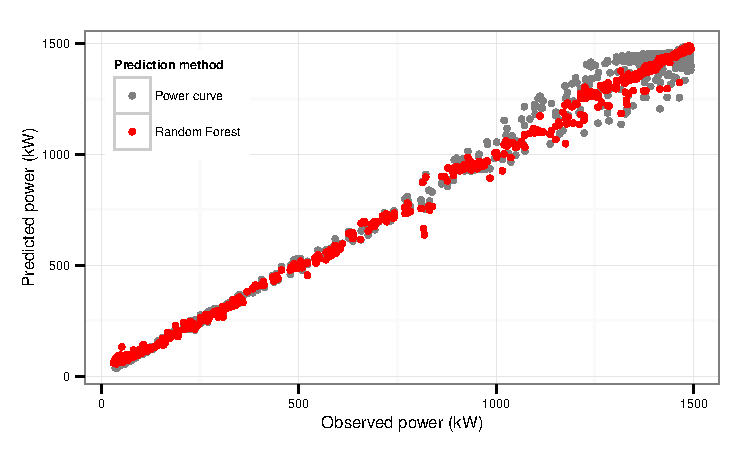
\includegraphics[width=5in,height=3in]{figure/PCversusRF-1} 

}

\caption[Comparison of the power predicted using the power curve and random forest methods]{Comparison of the power predicted using the power curve and random forest methods}\label{fig:PCversusRF}
\end{figure}


\end{knitrout}

We can get some error metrics for the different models, too:
\begin{knitrout}
\definecolor{shadecolor}{rgb}{0.969, 0.969, 0.969}\color{fgcolor}\begin{kframe}
\begin{alltt}
\hlkwd{GetErrorMetrics}\hlstd{(}\hlkwc{y} \hlstd{= PredPower}\hlopt{$}\hlstd{obs,}
                \hlkwc{ymod} \hlstd{= PredPower}\hlopt{$}\hlstd{PC)}
\end{alltt}
\begin{verbatim}
##                metric         type       value
## 1 Pearson Correlation Error metric          NA
## 2                RMSE Error metric    50.11007
## 3             Max(AE) Error metric   208.77220
## 4                 MAE Error metric    34.13595
## 5                 SAE Error metric 25772.64193
## 6                 SPE Error metric 12334.37403
\end{verbatim}
\begin{alltt}
\hlkwd{GetErrorMetrics}\hlstd{(}\hlkwc{y} \hlstd{= PredPower}\hlopt{$}\hlstd{obs,}
                \hlkwc{ymod} \hlstd{= PredPower}\hlopt{$}\hlstd{RF)}
\end{alltt}
\begin{verbatim}
##                metric         type        value
## 1 Pearson Correlation Error metric     0.998924
## 2                RMSE Error metric    24.813564
## 3             Max(AE) Error metric   181.096682
## 4                 MAE Error metric    14.210590
## 5                 SAE Error metric 10828.469240
## 6                 SPE Error metric  6043.756156
\end{verbatim}
\end{kframe}
\end{knitrout}

\section{Future developments}
Ideas for future developments of the \pkg{\pname} package should be sent to \href{mailto:andrew.clifton@nrel.gov}{andrew.clifton@nrel.gov}. Ideas that come with code snippets and functions that fit the framework of the package are very welcome!

Current ideas include:
\begin{itemize}
\item Create a wrapper, e.g. \code{ZTTrainTurbineModel()}, to train a zero-turbulence power curve for a specific site
\end{itemize}

%\bibliographystyle{jss}
\bibliography{../inst/examples/windenergy}

\end{document}
